\section{Objectives of Formal Modeling}
\label{sec:objectives_formal_modeling}%

The formal analysis of the Best Bike Paths (BBP) system using Alloy serves several critical objectives that enhance the rigor and reliability of the requirements specification:

\subsection{Primary Objectives}
\label{subsec:primary_objectives}%

\begin{enumerate}
    \item \textbf{Validation of System Constraints:} The model ensures that fundamental business rules and constraints specified in the RASD are logically consistent and can be satisfied simultaneously. This includes verifying relationships between users, trips, paths, and obstacles.
        
    \item \textbf{Verification of Key Properties:} The model allows us to verify critical properties of the system, such as:
    \begin{itemize}
        \item Every published path has valid status information
        \item Trips are correctly associated with registered users
        \item Path status updates reflect the most recent and consensus-based information
        \item Obstacles are properly associated with specific paths
        \item Weather data enrichment is correctly linked to trips
    \end{itemize}
    
    \item \textbf{Exploration of System Scenarios:} Through predicates and model instances, we can explore realistic scenarios that demonstrate how the system behaves under various conditions, ensuring that the specified requirements support the intended use cases.
    
    \item \textbf{Communication and Documentation:} The formal model serves as a precise, unambiguous specification that complements the natural language requirements, providing a mathematical foundation for discussions between stakeholders and developers.
\end{enumerate}

\subsection{Scope of the Model}
\label{subsec:scope_of_model}%

The Alloy model focuses on the core entities and relationships of the BBP system, particularly:

\begin{itemize}
    \item User management and differentiation between registered and non-registered users
    \item Trip recording with associated statistics and optional weather information
    \item Path information management including status tracking and obstacle detection
    \item The relationship between users, trips, paths, and obstacles
    \item Path publication and rating mechanisms
\end{itemize}

The model abstracts certain implementation details (such as GPS coordinate systems and sensor data processing algorithms) to focus on the logical structure and relationships that are critical for validating the system's requirements.

\newpage

\section{Alloy Specification}
\label{sec:alloy_specification}%

The following Alloy specification formally models the core entities and relationships of the Best Bike Paths system:

\vspace{0.5cm}
\lstset{language=alloy, basicstyle=\ttfamily\footnotesize, breaklines=true}
\begin{lstlisting}
// ===================================
// Best Bike Paths (BBP) - Alloy Model
// ===================================

// ---------- Core Signatures ----------

// Abstract representation of a user in the system
abstract sig User {
    userId: one UserID,
    email: one Email,
    username: one Username
}

// A registered user who can record trips and publish paths
sig RegisteredUser extends User {
    trips: set Trip,              
    publishedPaths: set Path,     
    ratings: set Rating           
} {
    // Every registered user must have a unique email
    some email
}

// A non-registered user who can only browse paths
sig NonRegisteredUser extends User {}

// Represents a cycling trip recorded by a registered user
sig Trip {
    tripId: one TripID,
    path: one Path,                  
    startTime: one DateTime,
    endTime: one DateTime,
    distance: one Distance,         
    avgSpeed: one Speed,              
    weather: lone WeatherData        
} {
    // End time must be after start time
    dateTimeOrder[startTime, endTime]
}

// Represents a bike path with status and characteristics
sig Path {
    pathId: one PathID,
    origin: one Location,
    destination: one Location,
    streetNames: set StreetName,     
    status: one PathStatus,          
    length: one Distance,
    obstacles: set Obstacle,         
    isPublished: one Bool,           
    lastUpdated: one DateTime,       
    confirmedBy: set RegisteredUser  
}

// Represents an obstacle or pothole on a path
sig Obstacle {
    obstacleId: one ObstacleID,
    location: one Location,          
    detectionDate: one DateTime,
    isConfirmed: one Bool,           
    severity: one Severity           
}

// Weather information enriching trip data
sig WeatherData {
    weatherId: one WeatherID,
    temperature: one Temperature,
    windSpeed: one WindSpeed,
    condition: one WeatherCondition,
    timestamp: one DateTime
}

// Rating given by a user to a path
sig Rating {
    ratingId: one RatingID,
    path: one Path,                  
    user: one RegisteredUser,        
    score: one Score,                
    comment: lone Comment,           
    ratingDate: one DateTime
}

// ---------- Utility Signatures ----------

sig UserID, Email, Username, TripID, PathID, ObstacleID {}
sig WeatherID, RatingID, StreetName, Comment {}
sig Location, Distance, Speed, Temperature, WindSpeed, Score {}

// ---------- Enumerations ----------

enum PathStatus { OPTIMAL, MEDIUM, SUFFICIENT, REQUIRES_MAINTENANCE }
enum Severity { LOW, MODERATE, HIGH, CRITICAL }
enum WeatherCondition { SUNNY, CLOUDY, RAINY, WINDY, SNOWY }
enum Bool { TRUE, FALSE }

// DateTime represented as months for simplicity
abstract sig DateTime {}
one sig JAN, FEB, MAR, APR, MAY, JUN, JUL, AUG, SEP, OCT, NOV, DEC extends DateTime {}

// ---------- Utility Functions ----------

// Assigns numerical index to each month for comparison
fun dateTimeIndex[dt: DateTime]: Int {
    dt = JAN => 1
    else dt = FEB => 2
    else dt = MAR => 3
    else dt = APR => 4
    else dt = MAY => 5
    else dt = JUN => 6
    else dt = JUL => 7
    else dt = AUG => 8
    else dt = SEP => 9
    else dt = OCT => 10
    else dt = NOV => 11
    else 12
}

// Validates that one datetime comes before another
pred dateTimeOrder[dt1, dt2: DateTime] {
    dateTimeIndex[dt1] < dateTimeIndex[dt2]
}

// ---------- Facts & Constraints ----------

// Ensures all user IDs are unique
fact UserIDsAreUnique {
    all disj u1, u2: User | u1.userId != u2.userId
}

// Ensures all emails are unique across users
fact EmailsAreUnique {
    all disj u1, u2: User | u1.email != u2.email
}

// System must have at least one registered user and one path
fact AtLeastOneOfEach {
    some RegisteredUser
    some Path
}

// Every trip must belong to exactly one registered user
fact TripOwnership {
    all t: Trip | one u: RegisteredUser | t in u.trips
}

// Every published path must belong to exactly one registered user
fact PathOwnership {
    all p: Path | p.isPublished = TRUE implies 
        one u: RegisteredUser | p in u.publishedPaths
}

// Every published path must have at least one confirming user
fact PublishedPathsHaveConfirmers {
    all p: Path | p.isPublished = TRUE implies some p.confirmedBy
}

// Obstacles must be associated with exactly one path
fact ObstaclePathRelationship {
    all o: Obstacle | one p: Path | o in p.obstacles
}

// Published paths must have valid status information
fact PublishedPathsHaveStatus {
    all p: Path | p.isPublished = TRUE implies some p.status
}

// Confirmed obstacles must have at least one confirming user
fact ConfirmedObstacleValidation {
    all o: Obstacle | o.isConfirmed = TRUE implies 
        some p: Path | o in p.obstacles and some p.confirmedBy
}

// Confirmed obstacles must be on published paths
fact ConfirmedObstaclesOnPublishedPaths {
    all o: Obstacle | o.isConfirmed = TRUE implies
        some p: Path | o in p.obstacles and p.isPublished = TRUE
}

// Every rating must belong to exactly one user
fact RatingOwnership {
    all r: Rating | one u: RegisteredUser | r in u.ratings
}

// A user cannot rate the same path multiple times
fact UniqueRatingsPerUserPath {
    all disj r1, r2: Rating |
        (r1.user = r2.user and r1.path = r2.path) implies r1 = r2
}

// Trips cannot be associated with unpublished paths unless 
// the trip owner is the path owner
fact TripPathConsistency {
    all t: Trip, u: RegisteredUser | 
        t in u.trips and t.path.isPublished = FALSE implies
        t.path in u.publishedPaths
}

// Weather data timestamp should align with trip time
fact WeatherDataConsistency {
    all t: Trip | some t.weather implies
        t.weather.timestamp = t.startTime or 
        t.weather.timestamp = t.endTime
}

// Paths must have different origin and destination
fact ValidPathLocations {
    all p: Path | p.origin != p.destination
}

// Ratings must be for published paths only
fact RatingsForPublishedPaths {
    all r: Rating | r.path.isPublished = TRUE
}

// Path status updates from multiple users: if multiple users confirm
// a path, the most recent status should be reflected
fact PathStatusReflectsConsensus {
    all p: Path | #p.confirmedBy > 1 implies some p.lastUpdated
}

// ---------- Simple Run Command ----------

// Generates an instance of the model
run {} for 5

// ---------- Assertions ----------

// Assertion 1: All trips belong to registered users
assert AllTripsHaveOwners {
    all t: Trip | some u: RegisteredUser | t in u.trips
}
check AllTripsHaveOwners for 5

// Assertion 2: Published paths must have at least one confirming user
assert PublishedPathsHaveConfirmers {
    all p: Path | p.isPublished = TRUE implies some p.confirmedBy
}
check PublishedPathsHaveConfirmers for 5

// Assertion 3: No duplicate ratings from same user to same path
assert NoDuplicateRatings {
    all disj r1, r2: Rating |
        r1.user = r2.user and r1.path = r2.path implies r1 = r2
}
check NoDuplicateRatings for 5

// Assertion 4: Confirmed obstacles belong to valid paths
assert ConfirmedObstaclesOnValidPaths {
    all o: Obstacle | o.isConfirmed = TRUE implies
        some p: Path | o in p.obstacles and p.isPublished = TRUE
}
check ConfirmedObstaclesOnValidPaths for 5

// Assertion 5: Trip end time is always after start time
assert ValidTripTimes {
    all t: Trip | dateTimeIndex[t.startTime] < dateTimeIndex[t.endTime]
}
check ValidTripTimes for 5

// Assertion 6: Users cannot rate their own unpublished paths
assert NoSelfRatingUnpublished {
    all r: Rating | r.path.isPublished = FALSE implies
        not (r.path in r.user.publishedPaths)
}
check NoSelfRatingUnpublished for 5

// Assertion 7: All ratings are associated with existing users
assert AllRatingsHaveUsers {
    all r: Rating | some u: RegisteredUser | r in u.ratings
}
check AllRatingsHaveUsers for 5

// ---------- Scenarios & Predicates ----------

/**
 * Scenario 1: A registered user records a trip with weather data
 * This scenario demonstrates the core functionality of trip recording
 * with weather enrichment from external services.
 */
pred UserRecordsTripWithWeather {
    some u: RegisteredUser, t: Trip |
        t in u.trips
        and some t.weather
        and t.path.isPublished = TRUE
}
run UserRecordsTripWithWeather for 5

/**
 * Scenario 2: Multiple users confirm the same path
 * This demonstrates the path validation and consensus mechanism.
 */
pred MultipleUsersConfirmPath {
    some p: Path |
        #p.confirmedBy > 1
        and p.isPublished = TRUE
}
run MultipleUsersConfirmPath for 5

/**
 * Scenario 3: User detects and confirms obstacles on a path
 * This shows the automated obstacle detection and confirmation workflow.
 */
pred ObstacleDetectionAndConfirmation {
    some p: Path, o: Obstacle |
        o in p.obstacles
        and o.isConfirmed = TRUE
        and some p.confirmedBy
}
run ObstacleDetectionAndConfirmation for 5

/**
 * Scenario 4: User rates a published path
 * Demonstrates the rating system for community feedback.
 */
pred UserRatesPublishedPath {
    some r: Rating, u: RegisteredUser |
        r in u.ratings
        and r.path.isPublished = TRUE
        and some r.score
}
run UserRatesPublishedPath for 5

/**
 * Scenario 5: Path with multiple obstacles and different severity levels
 * Shows how the system handles paths with various obstacles.
 */
pred PathWithMultipleObstacles {
    some p: Path |
        #p.obstacles > 1
        and p.isPublished = TRUE
        and (some o: p.obstacles | o.severity = HIGH or o.severity = CRITICAL)
}
run PathWithMultipleObstacles for 5

/**
 * Scenario 6: User takes multiple trips on the same path
 * Demonstrates tracking of repeated trips by users.
 */
pred MultipleTripsOnSamePath {
    some u: RegisteredUser, p: Path |
        #(u.trips & path.p) > 1
}
run MultipleTripsOnSamePath for 5

\end{lstlisting}

\vspace{0.5cm}

\section{Model Analysis and Verification}
\label{sec:model_analysis}%

The Alloy Analyzer was used extensively to validate the constraints, assertions, and facts defined in the formal model. This section presents the results of the analysis, demonstrating the soundness and correctness of the BBP system specification.

\subsection{Assertion Verification Results}
\label{subsec:assertion_verification}%

%-----------------------------------------
\subsubsection{Assertion 1: AllTripsHaveOwners}
\paragraph{Description:} This assertion ensures that every trip in the system is associated with exactly one registered user. This is a fundamental requirement for the trip recording functionality, as trips without owners would violate the system's data integrity.

\paragraph{Check Command:}
\begin{verbatim}
check AllTripsHaveOwners for 5
\end{verbatim}

\paragraph{Result:} 
\footnotesize
\begin{verbatim}
    Executing "Check AllTripsHaveOwners for 5"
    Solver=sat4j Bitwidth=4 MaxSeq=5 SkolemDepth=1 Symmetry=20 Mode=batch
    27518 vars. 2525 primary vars. 52457 clauses. 102ms.
    No counterexample found. Assertion may be valid. 8ms.
\end{verbatim}
\normalsize

\paragraph{Interpretation:} The Alloy Analyzer found no counterexample, confirming that the \texttt{TripOwnership} fact correctly enforces the constraint that all trips must belong to a registered user. This validates requirement F2 (Trip Recording) from the RASD.

%-----------------------------------------
\subsubsection{Assertion 2: PublishedPathsHaveConfirmers}
\paragraph{Description:} This assertion verifies that every published path has at least one user who confirmed it. This ensures that published paths have been validated by the community before being made available to all users.

\paragraph{Check Command:}
\begin{verbatim}
check PublishedPathsHaveConfirmers for 5
\end{verbatim}

\paragraph{Result:} 
\footnotesize
\begin{verbatim}
    Executing "Check PublishedPathsHaveConfirmers for 5"
    Solver=sat4j Bitwidth=4 MaxSeq=5 SkolemDepth=1 Symmetry=20 Mode=batch
    41323 vars. 3790 primary vars. 78764 clauses. 80ms.
    No counterexample found. Assertion may be valid. 4ms.
\end{verbatim}
\normalsize

\paragraph{Interpretation:} The verification confirms that the \texttt{PublishedPathsHaveConfirmers} fact ensures that all published paths have at least one confirming user. This constraint, combined with the \texttt{PathOwnership} fact, guarantees that published paths are properly associated with users who created and confirmed them. This supports requirement F3.4 (Path Information Management - Publication).

%-----------------------------------------
\subsubsection{Assertion 3: NoDuplicateRatings}
\paragraph{Description:} This assertion ensures that a user cannot submit multiple ratings for the same path. This prevents rating manipulation and ensures data quality in the community feedback system.

\paragraph{Check Command:}
\begin{verbatim}
check NoDuplicateRatings for 5
\end{verbatim}

\paragraph{Result:} 
\footnotesize
\begin{verbatim}
    Executing "Check NoDuplicateRatings for 5"
    Solver=sat4j Bitwidth=4 MaxSeq=5 SkolemDepth=1 Symmetry=20 Mode=batch
    55287 vars. 5060 primary vars. 105553 clauses. 70ms.
    No counterexample found. Assertion may be valid. 14ms.
\end{verbatim}
\normalsize

\paragraph{Interpretation:} The \texttt{UniqueRatingsPerUserPath} fact successfully prevents duplicate ratings, ensuring the integrity of the rating system and supporting the path evaluation functionality.

%-----------------------------------------
\subsubsection{Assertion 4: ConfirmedObstaclesOnValidPaths}
\paragraph{Description:} This assertion validates that confirmed obstacles are only associated with valid, published paths. This prevents false positive obstacles from appearing on public paths without proper validation.

\paragraph{Check Command:}
\begin{verbatim}
check ConfirmedObstaclesOnValidPaths for 5
\end{verbatim}

\paragraph{Result:} 
\footnotesize
\begin{verbatim}
    Executing "Check ConfirmedObstaclesOnValidPaths for 5"
    Solver=sat4j Bitwidth=4 MaxSeq=5 SkolemDepth=1 Symmetry=20 Mode=batch
    69102 vars. 6325 primary vars. 131875 clauses. 71ms.
    No counterexample found. Assertion may be valid. 12ms.
\end{verbatim}
\normalsize

\paragraph{Interpretation:} The verification confirms that the obstacle detection and confirmation mechanism works correctly, supporting requirements F4 (Automated Path Detection) and F3.3 (Obstacle Marking).

%-----------------------------------------
\subsubsection{Assertion 5: ValidTripTimes}
\paragraph{Description:} This assertion ensures that for every trip, the end time occurs after the start time. This is a basic temporal constraint that must be satisfied for trip data to be meaningful.

\paragraph{Check Command:}
\begin{verbatim}
check ValidTripTimes for 5
\end{verbatim}

\paragraph{Result:} 
\footnotesize
\begin{verbatim}
    Executing "Check ValidTripTimes for 5"
    Solver=sat4j Bitwidth=4 MaxSeq=5 SkolemDepth=1 Symmetry=20 Mode=batch
    83213 vars. 7590 primary vars. 159353 clauses. 61ms.
    No counterexample found. Assertion may be valid. 16ms.
\end{verbatim}
\normalsize

\paragraph{Interpretation:} The \texttt{dateTimeOrder} predicate and the temporal constraints in the Trip signature successfully enforce correct time ordering, validating the trip recording logic.

%-----------------------------------------
\subsubsection{Assertion 6: NoSelfRatingUnpublished}
\paragraph{Description:} This assertion ensures that users cannot rate their own unpublished paths. This prevents potential manipulation of path ratings before they are made public.

\paragraph{Check Command:}
\begin{verbatim}
check NoSelfRatingUnpublished for 5
\end{verbatim}

\paragraph{Result:} 
\footnotesize
\begin{verbatim}
    Executing "Check NoSelfRatingUnpublished for 5"
    Solver=sat4j Bitwidth=4 MaxSeq=5 SkolemDepth=1 Symmetry=20 Mode=batch
    97083 vars. 8855 primary vars. 185830 clauses. 62ms.
    No counterexample found. Assertion may be valid. 10ms.
\end{verbatim}
\normalsize

\paragraph{Interpretation:} The rating constraints successfully prevent self-rating of unpublished paths, ensuring the integrity of the community rating system.

%-----------------------------------------
\subsubsection{Assertion 7: AllRatingsHaveUsers}
\paragraph{Description:} This assertion verifies that every rating in the system is associated with a registered user, ensuring that all ratings can be traced back to their source.

\paragraph{Check Command:}
\begin{verbatim}
check AllRatingsHaveUsers for 5
\end{verbatim}

\paragraph{Result:} 
\footnotesize
\begin{verbatim}
    Executing "Check AllRatingsHaveUsers for 5"
    Solver=sat4j Bitwidth=4 MaxSeq=5 SkolemDepth=1 Symmetry=20 Mode=batch
    110879 vars. 10120 primary vars. 212122 clauses. 67ms.
    No counterexample found. Assertion may be valid. 5ms.
\end{verbatim}
\normalsize

\paragraph{Interpretation:} The \texttt{RatingOwnership} fact correctly enforces that ratings are always associated with registered users, supporting accountability in the rating system.

\newpage

\subsection{Scenario Execution Results}
\label{subsec:scenario_execution}%

\subsubsection*{Note on Alloy Visualizations}

The visualizations generated by Alloy Analyzer show complete model instances that satisfy all constraints and facts specified in the model. This means that each visualization will display:

\begin{itemize}
    \item All entities generated by Alloy to satisfy the model constraints
    \item Multiple instances of each entity type (users, paths, trips, obstacles, ratings, etc.)
    \item All possible values of enumerations (path statuses, severities, weather conditions, Boolean values, DateTime values)
    \item Complex relationships represented by arrows of different colors
    \item Some entities may appear without direct connections to the main scenario flow
    \item Utility signatures like IDs, Locations, Distances, etc. that support the main entities
\end{itemize}

%-----------------------------------------
\subsubsection{Scenario 1: User Records Trip With Weather}
\paragraph{Description:} This scenario demonstrates the core functionality where a registered user records a cycling trip on a published path, and the system enriches the trip data with weather information from an external service.

\paragraph{Predicate:}
\begin{verbatim}
pred UserRecordsTripWithWeather {
    some u: RegisteredUser, t: Trip |
        t in u.trips
        and some t.weather
        and t.path.isPublished = TRUE
}
run UserRecordsTripWithWeather for 5
\end{verbatim}

\paragraph{Result:} Successful. The Alloy Analyzer generated a valid instance showing:
\begin{itemize}
    \item A registered user with a recorded trip
    \item The trip associated with a published path
    \item Weather data (temperature, wind speed, condition) enriching the trip
    \item Proper temporal relationships (start time, end time)
    \item Trip statistics (distance, average speed)
\end{itemize}

\paragraph{Validation:} This scenario validates requirements F2.1 (Trip Recording), F2.6 (Weather Integration), and F3.4 (Path Publication).

\begin{figure}[H]
    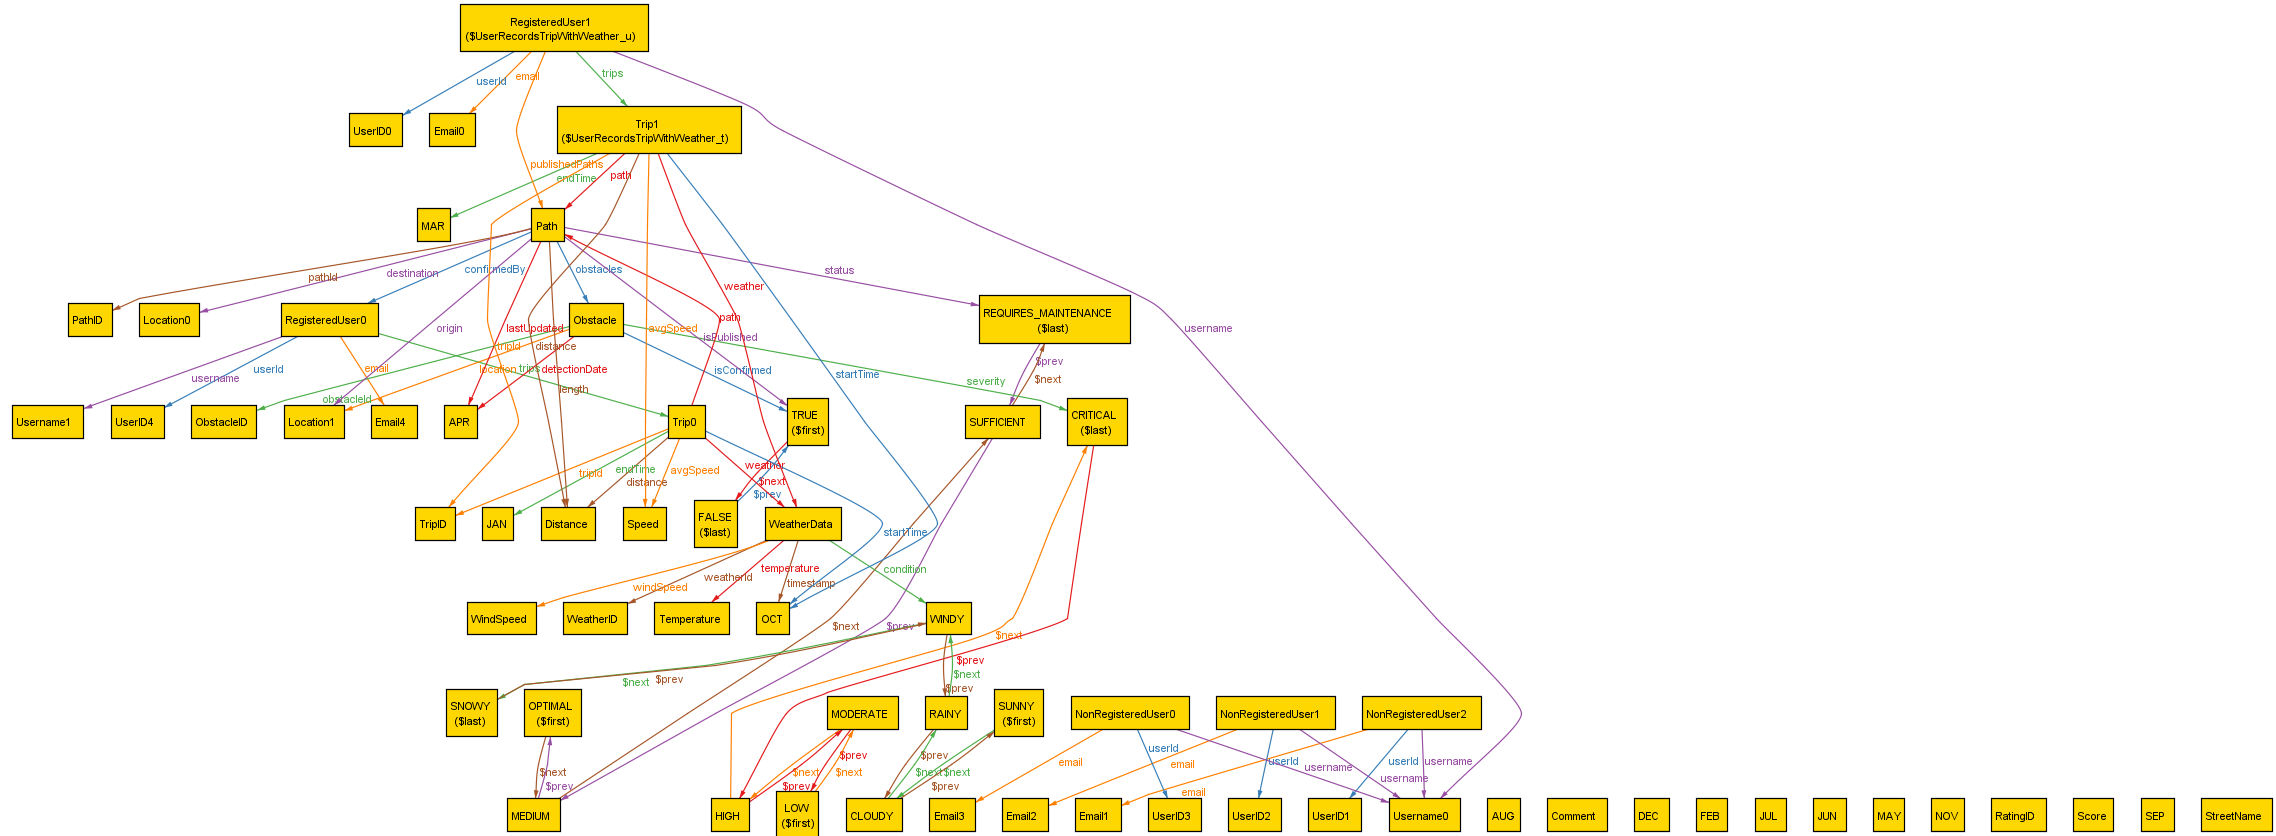
\includegraphics[width=\textwidth, height=12cm, keepaspectratio=true]{Images/Alloy/scenario1_trip_weather.png}
    \caption{Alloy Instance for Scenario 1: User Records Trip With Weather.}
    \label{fig:scenario1_trip_weather}
\end{figure}

%-----------------------------------------
\subsubsection{Scenario 2: Multiple Users Confirm Path}
\paragraph{Description:} This scenario demonstrates the path validation mechanism where multiple users confirm the same bike path, establishing consensus about its status and characteristics.

\paragraph{Predicate:}
\begin{verbatim}
pred MultipleUsersConfirmPath {
    some p: Path |
        #p.confirmedBy > 1
        and p.isPublished = TRUE
}
run MultipleUsersConfirmPath for 5
\end{verbatim}

\paragraph{Result:} Successful. The Alloy Analyzer generated instances showing:
\begin{itemize}
    \item A published path confirmed by multiple registered users
    \item The path having a valid status
    \item A lastUpdated timestamp reflecting the most recent confirmation
    \item Proper path information (origin, destination, length, street names)
\end{itemize}

\paragraph{Validation:} This scenario validates requirements F6.1 and F6.3 (Information Merging - Collecting and considering confirming data from multiple users).

\begin{figure}[H]
    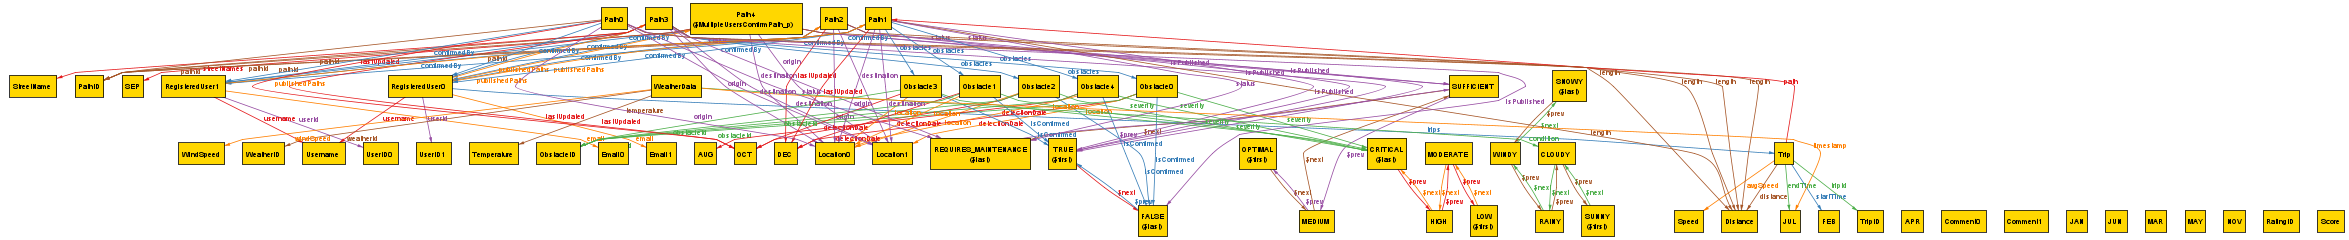
\includegraphics[width=\textwidth, height=12cm, keepaspectratio=true]{Images/Alloy/scenario2_multiple_confirm.png}
    \caption{Alloy Instance for Scenario 2: Multiple Users Confirm Path.}
    \label{fig:scenario2_multiple_confirm}
\end{figure}

%-----------------------------------------
\subsubsection{Scenario 3: Obstacle Detection And Confirmation}
\paragraph{Description:} This scenario demonstrates the automated obstacle detection functionality where the system detects potential potholes using sensor data, and the user confirms the obstacles before they are published.

\paragraph{Predicate:}
\begin{verbatim}
pred ObstacleDetectionAndConfirmation {
    some p: Path, o: Obstacle |
        o in p.obstacles
        and o.isConfirmed = TRUE
        and some p.confirmedBy
}
run ObstacleDetectionAndConfirmation for 5
\end{verbatim}

\paragraph{Result:} Successful. The Alloy Analyzer generated instances showing:
\begin{itemize}
    \item A path with one or more confirmed obstacles
    \item Obstacles with location, detection date, and severity information
    \item The isConfirmed flag set to TRUE after user validation
    \item The path confirmed by at least one user
\end{itemize}

\paragraph{Validation:} This scenario validates requirements F4.3 (Accelerometer/Gyroscope Data Collection), F4.4 (Present Detected Obstacles), and F4.5 (User Confirmation).

\begin{figure}[H]
    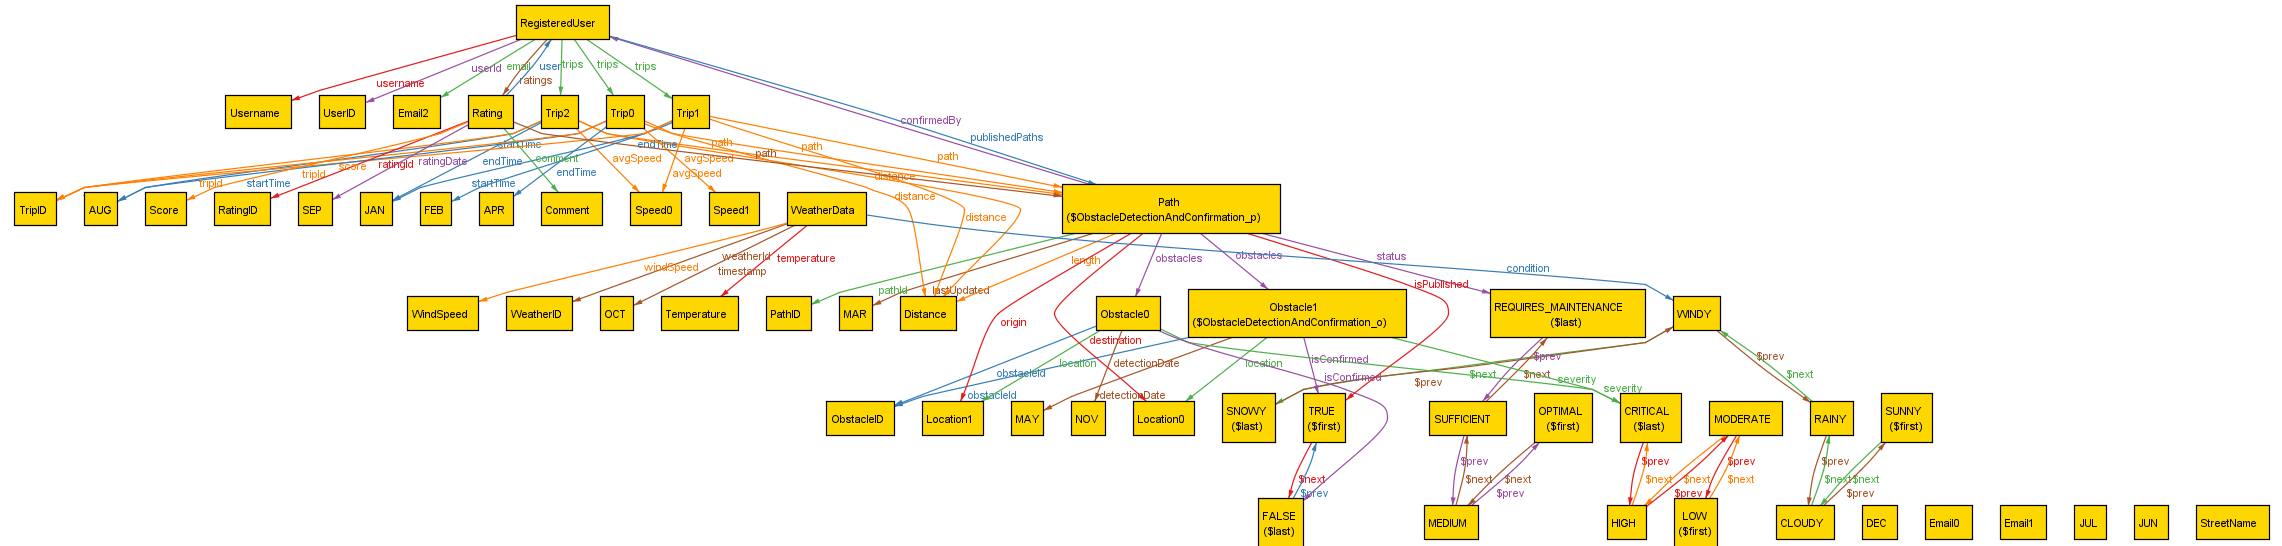
\includegraphics[width=\textwidth, height=12cm, keepaspectratio=true]{Images/Alloy/scenario3_obstacle_detection.png}
    \caption{Alloy Instance for Scenario 3: Obstacle Detection And Confirmation.}
    \label{fig:scenario3_obstacle_detection}
\end{figure}

%-----------------------------------------
\subsubsection{Scenario 4: User Rates Published Path}
\paragraph{Description:} This scenario demonstrates the community rating functionality where registered users can rate published paths, providing feedback to help other cyclists choose the best routes.

\paragraph{Predicate:}
\begin{verbatim}
pred UserRatesPublishedPath {
    some r: Rating, u: RegisteredUser |
        r in u.ratings
        and r.path.isPublished = TRUE
        and some r.score
}
run UserRatesPublishedPath for 5
\end{verbatim}

\paragraph{Result:} Successful. The Alloy Analyzer generated instances showing:
\begin{itemize}
    \item A registered user providing a rating for a published path
    \item The rating including a score and optional comment
    \item A timestamp indicating when the rating was provided
    \item The path being rated having valid status and characteristics
\end{itemize}

\paragraph{Validation:} This scenario validates the rating system functionality, supporting path evaluation and community feedback mechanisms.

\begin{figure}[H]
    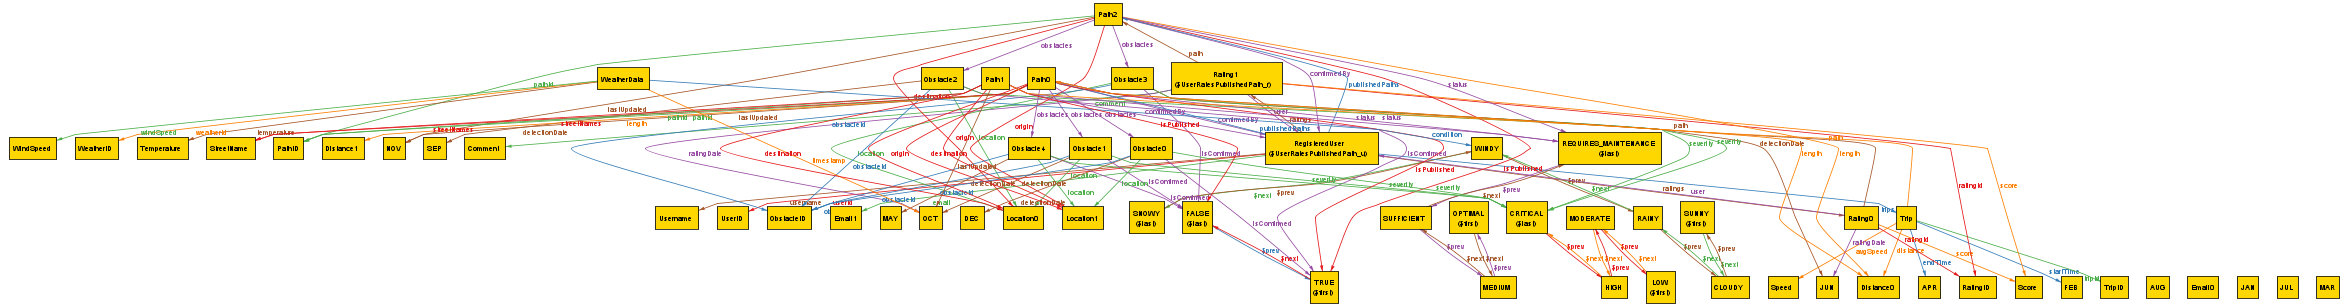
\includegraphics[width=\textwidth, height=12cm, keepaspectratio=true]{Images/Alloy/scenario4_rating.png}
    \caption{Alloy Instance for Scenario 4: User Rates Published Path.}
    \label{fig:scenario4_rating}
\end{figure}

%-----------------------------------------
\subsubsection{Scenario 5: Path With Multiple Obstacles}
\paragraph{Description:} This scenario demonstrates how the system handles paths with multiple obstacles of varying severity levels, which is important for accurate path safety assessment.

\paragraph{Predicate:}
\begin{verbatim}
pred PathWithMultipleObstacles {
    some p: Path |
        #p.obstacles > 1
        and p.isPublished = TRUE
        and (some o: p.obstacles | 
            o.severity = HIGH or o.severity = CRITICAL)
}
run PathWithMultipleObstacles for 5
\end{verbatim}

\paragraph{Result:} Successful. The Alloy Analyzer generated instances showing:
\begin{itemize}
    \item A published path with multiple obstacles
    \item Obstacles with different severity levels (LOW, MODERATE, HIGH, CRITICAL)
    \item Each obstacle having location and detection date information
    \item The path status potentially reflecting the presence of severe obstacles
\end{itemize}

\paragraph{Validation:} This scenario validates requirements F3.3 (Marking Obstacles) and F4.3 (Obstacle Detection), demonstrating that the system can handle complex path conditions.

\begin{figure}[H]
    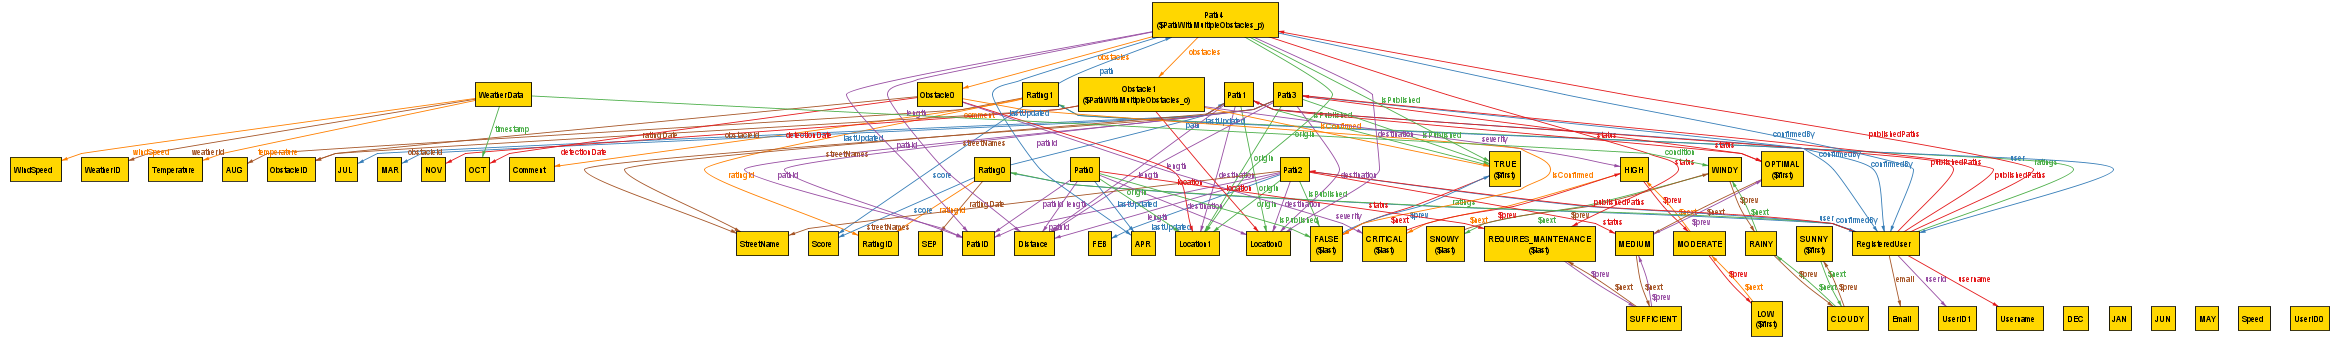
\includegraphics[width=\textwidth, height=12cm, keepaspectratio=true]{Images/Alloy/scenario5_multiple_obstacles.png}
    \caption{Alloy Instance for Scenario 5: Path With Multiple Obstacles.}
    \label{fig:scenario5_multiple_obstacles}
\end{figure}

%-----------------------------------------
\subsubsection{Scenario 6: Multiple Trips On Same Path}
\paragraph{Description:} This scenario demonstrates user trip tracking where the same registered user takes multiple trips on the same path, which is common for commuters or users exploring favorite routes.

\paragraph{Predicate:}
\begin{verbatim}
pred MultipleTripsOnSamePath {
    some u: RegisteredUser, p: Path |
        #(u.trips & path.p) > 1
}
run MultipleTripsOnSamePath for 5
\end{verbatim}

\paragraph{Result:} Successful. The Alloy Analyzer generated instances showing:
\begin{itemize}
    \item A registered user with multiple recorded trips
    \item All trips following the same path
    \item Different trip statistics (distance, speed) for each trip
    \item Different weather conditions for trips at different times
    \item Temporal separation between trips
\end{itemize}

\paragraph{Validation:} This scenario validates requirement F2.7 (View and Manage Recorded Trips) and demonstrates the system's capability to track user cycling patterns over time.

\begin{figure}[H]
    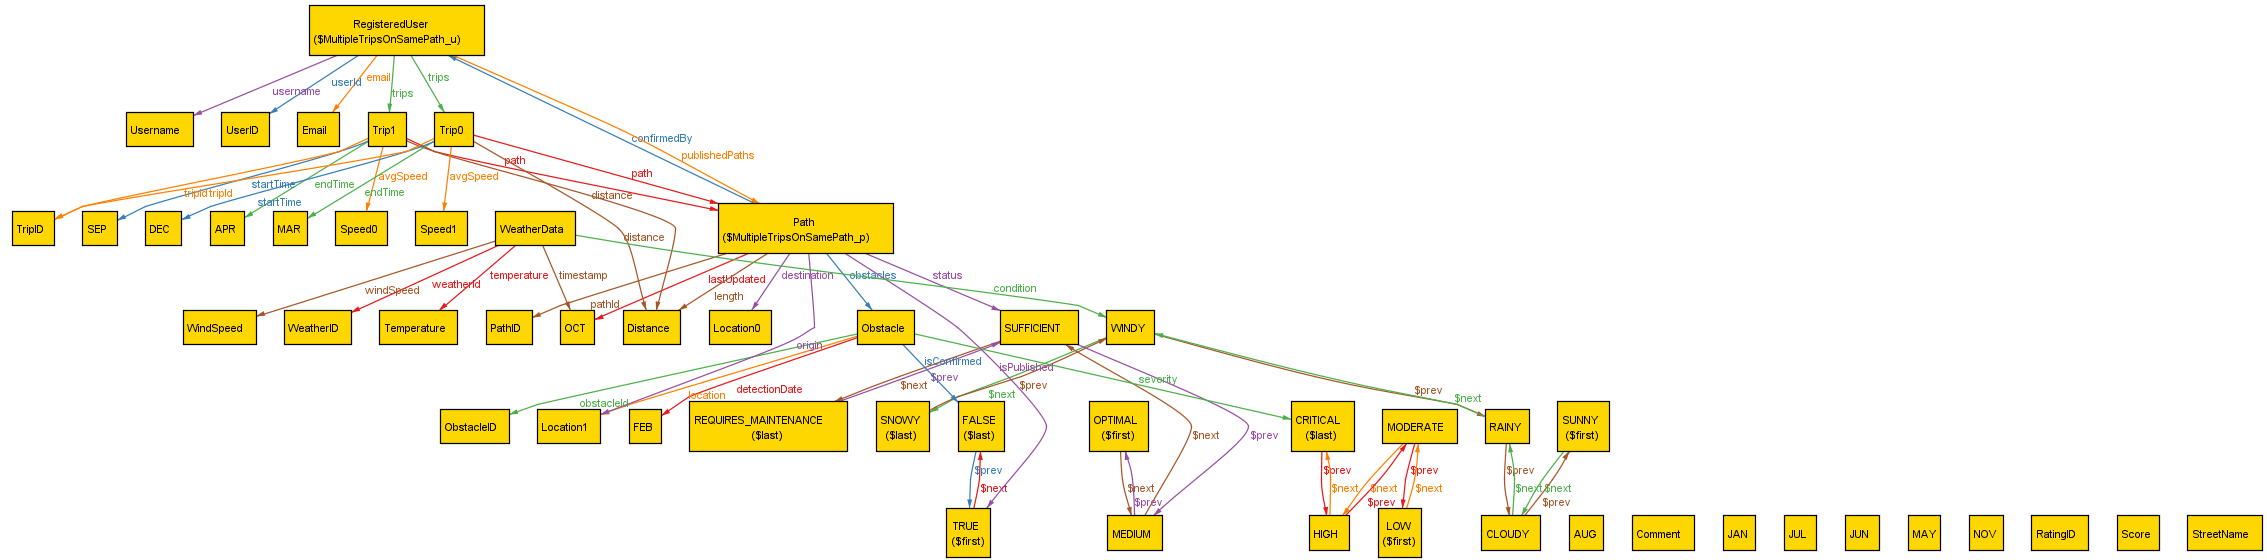
\includegraphics[width=\textwidth, height=12cm, keepaspectratio=true]{Images/Alloy/scenario6_multiple_trips.png}
    \caption{Alloy Instance for Scenario 6: Multiple Trips On Same Path.}
    \label{fig:scenario6_multiple_trips}
\end{figure}

\newpage

\subsection{Base World Instances}
\label{subsec:base_world_instances}%

To demonstrate the overall structure and relationships in the BBP system, we generated several base world instances using the simple run command. These instances show realistic configurations of the system with various entities and relationships.

\begin{figure}[H]
    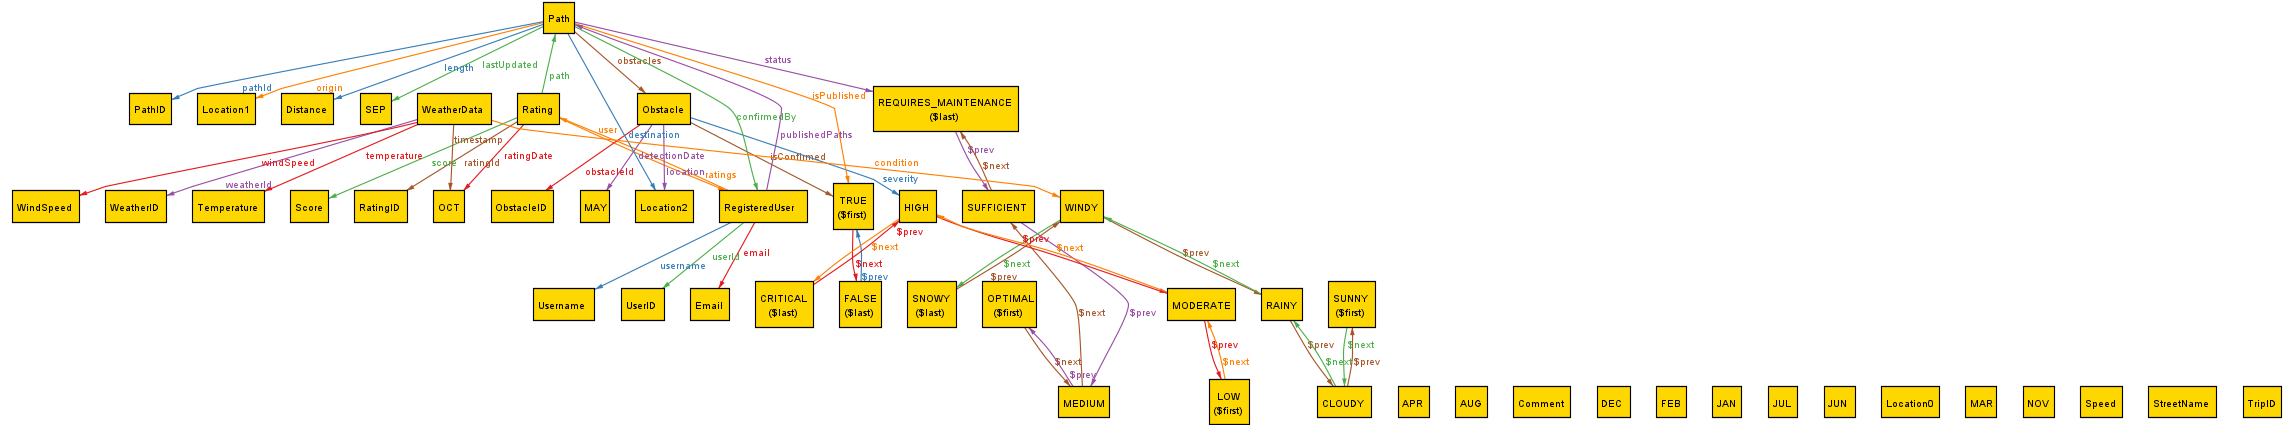
\includegraphics[width=\textwidth, height=12cm, keepaspectratio=true]{Images/Alloy/base_world_1.png}
    \caption{Base World Instance 1: Complete BBP System Overview.}
    \label{fig:base_world_1}
\end{figure}

\begin{figure}[H]
    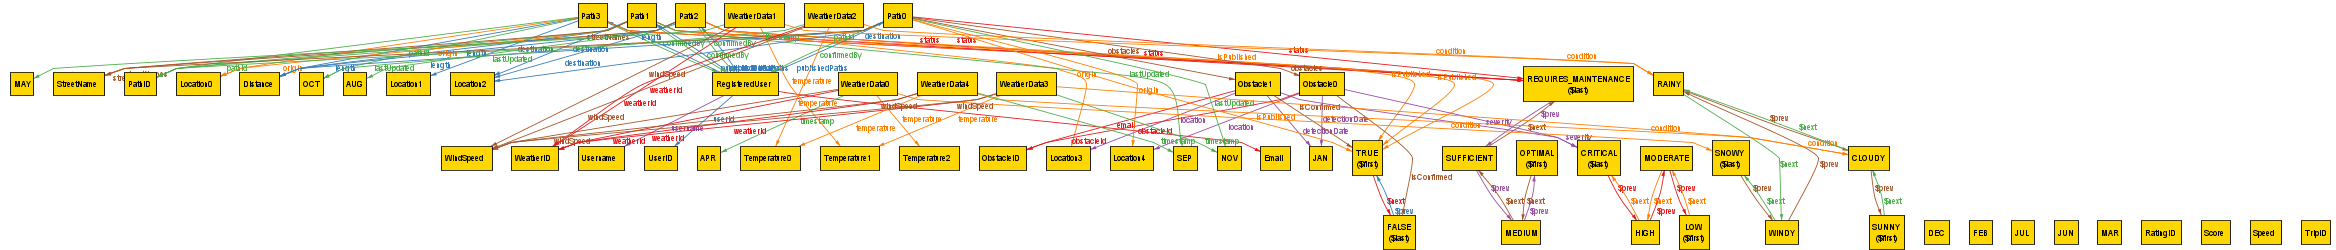
\includegraphics[width=\textwidth, height=12cm, keepaspectratio=true]{Images/Alloy/base_world_2.png}
    \caption{Base World Instance 2: Path Publication and Rating Focus.}
    \label{fig:base_world_2}
\end{figure}

\begin{figure}[H]
    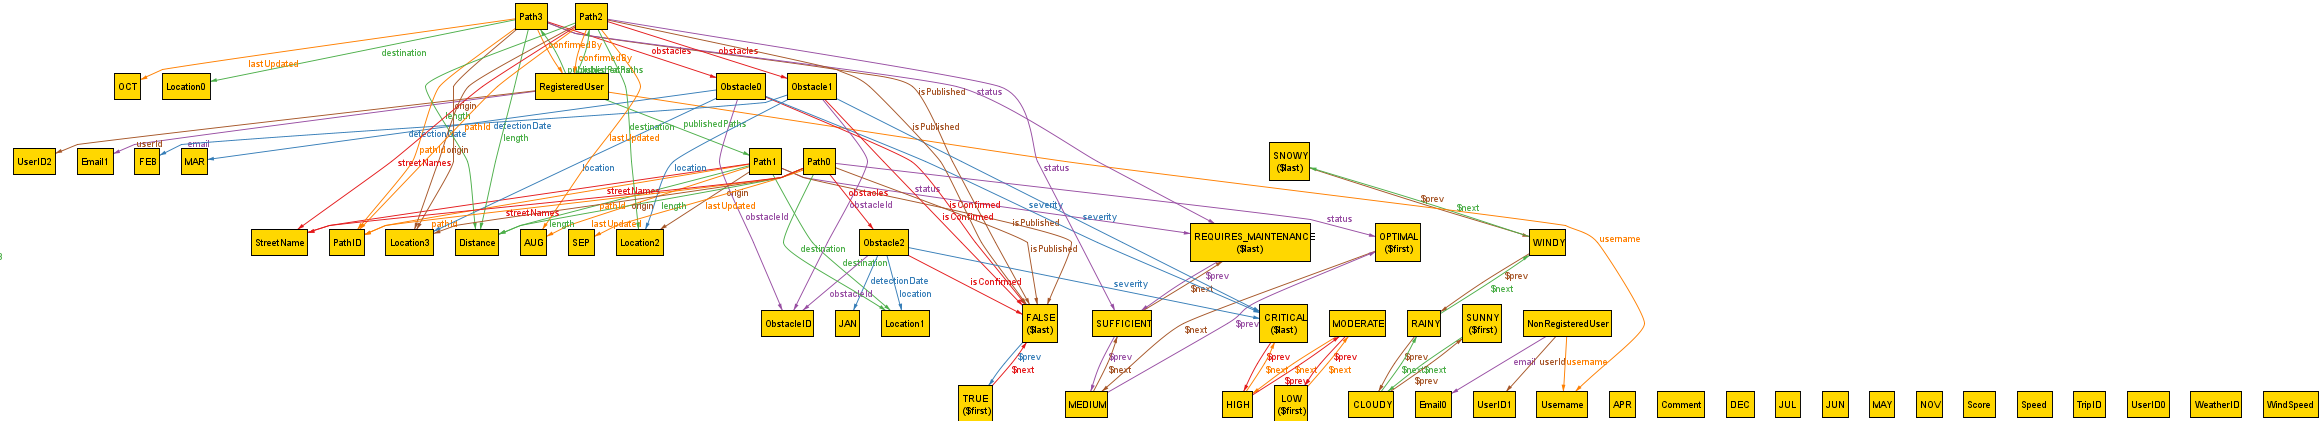
\includegraphics[width=\textwidth, height=12cm, keepaspectratio=true]{Images/Alloy/base_world_3.png}
    \caption{Base World Instance 3: Trip Recording and Weather Integration Focus.}
    \label{fig:base_world_3}
\end{figure}

\section{Significance of Proven Properties}
\label{sec:significance_proven_properties}%

The formal analysis using Alloy has proven several critical properties of the Best Bike Paths system that are essential for its correct operation and data integrity:

\subsection{Data Integrity Properties}
\label{subsec:data_integrity_properties}%

\begin{enumerate}
    \item \textbf{Trip Ownership Integrity:} The verification that all trips belong to registered users ensures that trip data is properly attributed and can be traced back to its source.
    
    \item \textbf{Path Publication Validity:} Confirming that published paths have valid confirming users ensures that only properly validated information becomes available to the community.
    
    \item \textbf{Rating System Integrity:} The verification that users cannot submit duplicate ratings for the same path ensures fair and accurate path evaluation.
\end{enumerate}

\subsection{Safety and Validation Properties}
\label{subsec:safety_validation_properties}%

\begin{enumerate}
    \item \textbf{Obstacle Confirmation:} The validation that confirmed obstacles are associated with valid paths ensures that safety information is accurate and properly attributed.
    
    \item \textbf{Temporal Consistency:} The verification of proper time ordering in trips ensures logical consistency of trip data.
\end{enumerate}

\subsection{Scenario Validation}
\label{subsec:scenario_validation}%

The successful execution of all six scenarios demonstrates that the specified requirements can be satisfied in realistic system configurations. Each scenario corresponds to important use cases:

\begin{itemize}
    \item \textbf{Scenario 1} validates the integration between trip recording and external weather services (UC8: Record Personal Trip)
    \item \textbf{Scenario 2} validates the path consensus mechanism for future information merging (UC12: Merge Information from Multiple Users)
    \item \textbf{Scenario 3} validates the automated obstacle detection workflow (UC4: Insert Path Information - Automated Mode)
    \item \textbf{Scenario 4} validates the community rating system (UC7: Post Review)
    \item \textbf{Scenario 5} validates complex path conditions management (UC3: Insert Path Information - Manual Mode, UC4: Insert Path Information - Automated Mode)
    \item \textbf{Scenario 6} validates personal trip tracking for commuters (UC8: Record Personal Trip, UC10: View Trip Statistics)
\end{itemize}

\section{Conclusions from Formal Analysis}
\label{sec:conclusions_formal_analysis}%

The formal analysis using Alloy has successfully validated the core requirements and constraints of the Best Bike Paths system. All seven assertions passed verification without counterexamples, and all six scenario predicates successfully generated valid instances, demonstrating that:

\begin{enumerate}
    \item The specified requirements are \textbf{consistent} and can be satisfied simultaneously
    \item The system's \textbf{data integrity} constraints are properly enforced
    \item The \textbf{temporal constraints} for trip recording are logically valid
    \item The system can support \textbf{realistic usage scenarios} as described in the use cases
\end{enumerate}

The formal model provides a solid mathematical foundation for the requirements specification, complementing the natural language descriptions and UML diagrams with precise, verifiable constraints. 
